\chapter{Implementación}

\section{Software}

Para diseñar una interfaz de usuario real, en la que poder basarme para luego representarla mediante HTML y CSS, se utilizan diversos programas de diseño web.

\begin{itemize}

\item \textbf{Sketch}: Sketch es una aplicación de diseño vectorial, que te permite diseñar interfaces para aplicaciones móviles o web de una manera sencilla y con una gran potencia.
\item \textbf{Illustrator}: Esta herramienta de adobe tan famosa, te permite el diseño de logotipos de forma vectorial,
\item \textbf{Spectrum}: Programa sencillo que te permite crear paletas de colores, de forma que puedas seleccionar colores complementarios o de gama monocromática y utilizarlos para la interfaz de la aplicación.

\end{itemize}

\section{Tecnologías}

Para la realización de la aplicación web, se ha llevado a cabo un análisis de las tecnologías disponibles, y se han seleccionado las que mejor se adaptaban a las necesidades del proyecto.

\subsection{Front-End(Cliente)}

Las dos principales e indispensables tecnologías que se usan para la parte del cliente son el lenguaje de etiquetas HTML5 y las hojas de etilos CSS3. Estas son dos de las tecnologías fundamentales en las que se basa el desarrollo web.

 \vspace{5 mm}

 Con la finalidad de conseguir una apariencia cuidada e intuitiva del sitio web, sin la necesidad de crear las hojas de estilos propias, se planteó la idea de usar el framework Bootstrap. Finalmente debido al objetivo de personalizar al máximo la apariencia de la web, se descartó Bootstra y se optó por añadir clases propias mediante css.

\vspace{5 mm}

Para maquetar el sitio web con CSS3 de forma más rápida y refactorizable se utiliza \textbf{Sass}. Sass es un lenguaje de preprocesado de CSS, que permite escribir CSS de forma más cómoda, posibilitando declarar variables,mixins, herencia de clases, etc. Hay diversas formas de utilizar Sass en tu proyecto. Mediante un programa como Prepros, mediante un automatizador de tareas como Grunt, o mediante un terminal con los comandos de Sass. Para el proyecto yo he optado usar el terminal para ejecutar Sass, ya que su ejecución es mucho más ligera y consume menos RAM que con programas como Prepros. Para que empezar a usar Sass en el proyecto, dentro de nuestra carpeta padre donde se encuentre el css, se crea una carpeta sass donde se incluirán todos los ficheros .scss. Con el terminal situado en la carpeta padre escribimos sass --watch sass(nombre de la carpeta donde se encuentran los ficheros .scss). Al compilarlo, generará un fichero style.css que será la hoja de estilo a usar.

\vspace{5 mm}

Para añadir el dinamismo a la web, se ha optado por utilizar un framework de Javascript como \textbf{JQuery} que permite simplificar la manera de interactuar con los documentos HTML, manipular el DOM, desarrollar animaciones y agregar peticiones AJAX. Además de que JQuery es software libre.

\vspace{5 mm}

Como última tecnología Front-End se utiliza la API de Google Maps, indispensable para el sitio web ya que la principal proposición de valor de la aplicación es la geolocalización de recetas, y para su representación necesitamos la API de Google.


\subsection{Back-End(Servidor)}

Después de barajar diversos lenguajes para desarrollar el back-end de la aplicación, finalmente se eleigió PHP. Además de ser el lenguaje más utlizado para el desarrollo web, es uno de los lenguajes más potentes y flexibles, pudiendo ser utilizado en la mayoría de los servidores web y sistemas operativos. Además PHP esta publicado bajo licencia de software libre, por lo que no supone ningun coste.


\vspace{5 mm}

Para montar la arquitectura MVC en la aplicación, se utiliza el framwework Laravel. Laravel agiliza el desarrollo de las aplicaciones web, permitiendo multitud de funcionalidades. Con este framework, desarrollado de forma elegante y simple se evita la creación de código espagueti, faciltando su refactorización y/o su modificación. Algunas de las carácterísticas de Laravel: 


\begin{itemize}

\item \textbf{Plantillas}: Laravel utiliza platillas Blade. Blade permite tener un sitema de vistas modular de forma que se tenga que repetir la menor cantidad de código. Para ello se genera una plantilla base o layout, que es donde se representa la estructura de la web y se volcará el contenido para cada página. Mediante la directiva include(nombre\_template), se podrá incluir una vista parcial de contenido HTML, esta directiva se utiliza para contenido que no cambia por ejemplo para incluir la cabecera o el footer de la aplicación. Luego mediante la sentencia yield(nombre\_template) permitiremos crear una futura sección en el HTML que se definirá en las vistas que son heredadas de este template. Mediante la sentencia extends(nombre\_template) le diremos a Laravel que vistas se van a usar como futuras secciones. Con estas sentencias se conseguirá volcar el contenido especifíco para cada página de la web duplicando el menor numero de codigo HTML y de forma más modular.

\item \textbf{ORM}: Es una implementación de registro activo para trabajar con la base de datos de forma que cada tabla de la base de datos tiene un Modelo correspondiente asociado con el mismo nombre. Esta implementación te permite también métodos predefinidos para llamar a la base de datos como save(),create(),get(),find().

\item \textbf{Caché}: Laravel, cuenta con un robusto sistema de caché, el cual se puede ajustar, para que se produzca una carga rápida de la web y generar una mejor experiencia al usuario.

\item \textbf{MiddleWare}: Usa HTTP Middleware, que proporcionan un correcto mecanismo para filtrar las peticiones en la aplicación. Un ejemplo de middleware que incluye laravel, es el usado para verificar si el usuario esta autenticado en la aplicación.

\end{itemize}

\vspace{5 mm}

Para la base de datos, se utiliza el sistema de gestión relacional MySQL, ya que es uno de los sistemas más utilizados y con mayor documentación para el desarrollo web. Además, de la perfecta integración con Laravel.

\subsection{Estructura de la aplicación}

Para comenzar a desarrollar el proyecto, primero se debe instalar Laravel. Para ello se utiliza un manejador de dependencias como composer que nos permite instalar los paquetes y librerías de forma automática sin la necesidad de hacerlo de forma manual. Mediante nuestro terminal escribimos el siguiente código para instalar composer en el ordenador: curl -sS https://getcomposer.org/installer | php. Una vez instalado, para generar un proyecto con laravel escribimos en el terminal el siguiente comando: composer create-project laravel/laravel nombre-proyecto.

\vspace{5 mm}

\begin{figure}
\begin{center}
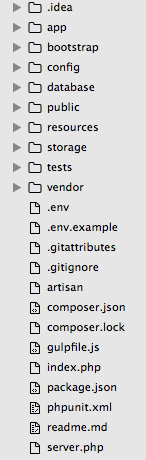
\includegraphics[width=1.0\textwidth]{imagenes/estructura-laravel.png}
\caption{Proyecto de Laravel}
\label{laravel}
\end{center}
\end{figure}

Si vamos a la carpeta raiz con la que creamos el proyecto se observa que dentro composer ha generado una estructura de directorios(figura \ref{laravel}) que es como organiza Laravel el código de la aplicación. A continuación se detallan brevemente cada una de ellas:


\begin{itemize}

\item \textbf{app}: el directorio app es donde se encontrará la mayor parte del código personal del back-end de la aplicación. Desde los modelos de datos de la aplicación, hasta los controladores pasando por el middleware.

\item \textbf{config}: aqui se encuentran los ficheros de configuración de Laravel y de la aplicación. Por ejemplo en el fichero app.php se especifican parametros tales como la zona horaria y el idioma de la aplicación. También se definen los providers, que son cada uno de los objetos o instancias que se cargarán en el proyecto. 

\item \textbf{database}: aquí se encuentran todos los ficheros relacionados con la base de datos de la aplicación. Dentro encontramos tres subdirectorios:

- factories: aquí se incluyen los ficheros que generan automaticamente nuevos datos en tu base de datos para testear la aplicación, sin necesidad de generarlos manualmente.

- migrations: las migraciones son un tipo de control de versiones para la base de datos. A través de estos ficheros se puede modificar la base de datos.

- seeds: permiten poblar la base de datos con datos de prueba. Los seeds pueden utilizar factories para poblar la base de datos o introudcirlos manualmente.

\item \textbf{public}: en este directorio se encuentran los directorios con ficheros estáticos como son las hojas de estilo(css), los ficheros javascript(js) y las imágenes(images).

\item \textbf{resources}: en resource encontramos subdirectorios donde se encuentran las vistas  en formato blade.php de la aplicación(views) y los archivos de idiomas de la aplicación, para poder pasar de un idioma a otro en la aplicación(lang).

\item \textbf{storage}: se encuentran varios subdirectorios que contiene el cache de la aplicación, sesiones, etc.

\item \textbf{vendor}: este directorio contiene todo el core de Laravel y los componentes instalados.

\end{itemize}

\begin{figure}
\begin{center}
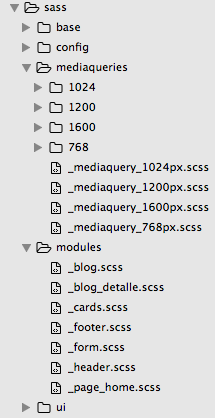
\includegraphics[width=1.0\textwidth]{imagenes/estructura-sass.png}
\caption{Estructura Sass}
\label{sass}
\end{center}
\end{figure}

\textbf{Estructura Sass} 

Como se comenta previamente, se utiliza Sass para maquetar la web. Este lenguaje de preprocesado de Css te permite organizar el ccs y hacerlo más modular de forma que puedes generar varios ficheros .scss y compilarlos en un único fichero css que es el que se utilizará en la aplicación. Para ello uso una carpeta sass que se incluye en la carpeta public del proyecto donde incluyo todos los directorios con los ficheros sass. Una de las formas de refactorizar más el código Sass, es generar un fichero .scss para cada página web de la aplicación de modo que en futuros cambios resulte todavía más sencillo modificar el estilo. Como se observa en la figura \ref{sass} la estructura sass es al siguiente:


\begin{itemize}

\item \textbf{base}: en el directorio base se encuentran los ficheros scss con los elementos más básicos de la aplicación. Las tipografías usadas, los formatos de texto de los encabezados y párrafos, etc.

\item \textbf{config}: en este directorio encontramos los siguientes ficheros.

- variables: scss donde se declaran las variables que se usan en las hojas de estilo tales como colores de la aplicación, las fuentes usadas.

- functions: aquí se encuentran los mixins de sass que se pueden utilizar. Los mixins no son más que funciones que te permiten reutilizar estilos.

- animations: en este directorio se incluyen los ficheros scss con animaciones hechas con css incluidas en la aplicación.

\item \textbf{ui}: en el directorio ui(user interface) se incluyen los ficheros scss que modifiquen las propiedades css de elementos de la interfaz gráfica de la aplicación como botones,formularios, etc.

\item \textbf{modules}: debido a que la aplicación esta basada en la filosofía mobile first en esta carpeta se incluyen todos lo ficheros scss de las páginas de la aplicación en resolución móvil(de 0 a 768px de resolución de pantalla).

\item \textbf{mediaqueries}: en esta carpeta se incluyen los ficheros scss para las resoluciones de tablet y ordenador de escritorio. Para esta resolución se han marcado las resolución de 768px a 1024px(tablet) y para escritorio las resoluciones de 1024px a 1600px y mayores de 1600px. Para cada resolución habrá un subdirectorio con el nombre de la resolución donde se incluirán sus ficheros scss correspondientes.


\end{itemize}

\vspace{5 mm}

\section{Sprints}

Una instalado el framework Laravel y comprendida su estructura se procede a desarrollar la aplicación. Para realizar el proyecto, como se especifica previamente se utiliza la metodología Scrum. El proyecto se divide en los siguientes sprints:


\subsection{Diseño de la interfaz}

\begin{figure}
\begin{center}
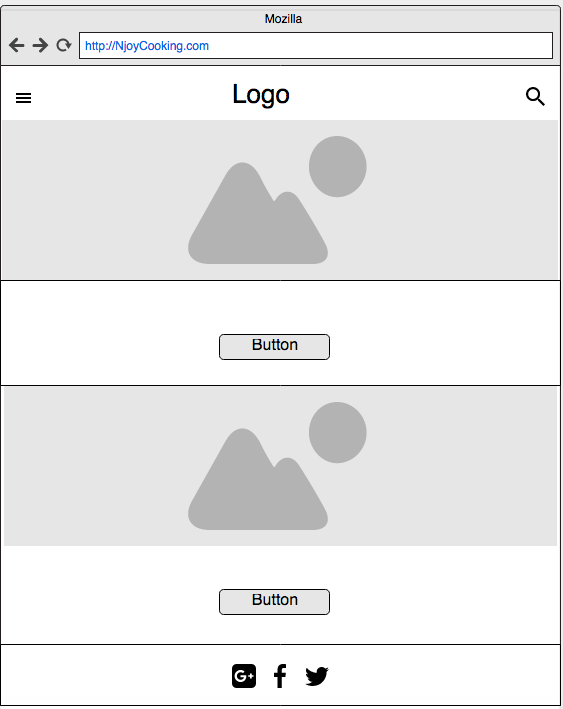
\includegraphics[width=1.0\textwidth]{imagenes/landing.png}
\caption{Landing}
\label{landing}
\end{center}
\end{figure}

\begin{figure}
\begin{center}
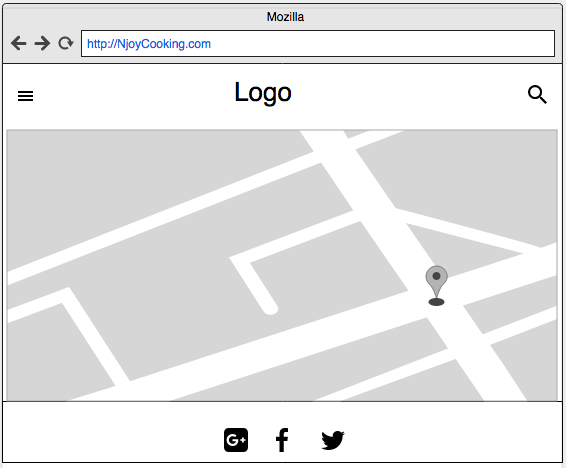
\includegraphics[width=1.0\textwidth]{imagenes/mapa.png}
\caption{Mapa}
\label{mapa}
\end{center}
\end{figure}

\begin{figure}
\begin{center}
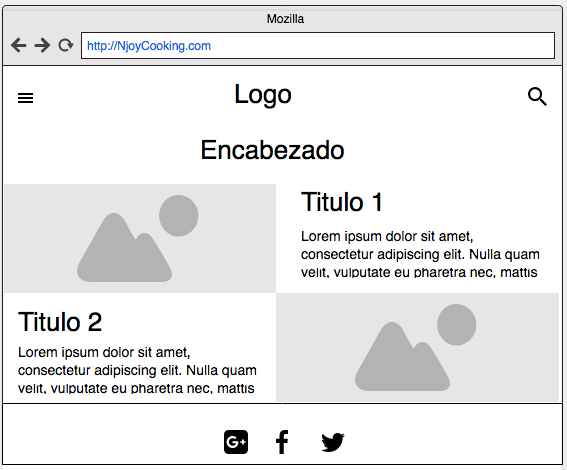
\includegraphics[width=1.0\textwidth]{imagenes/listado-blog.png}
\caption{Listado de noticias}
\label{listado-blog}
\end{center}
\end{figure}

\begin{figure}
\begin{center}
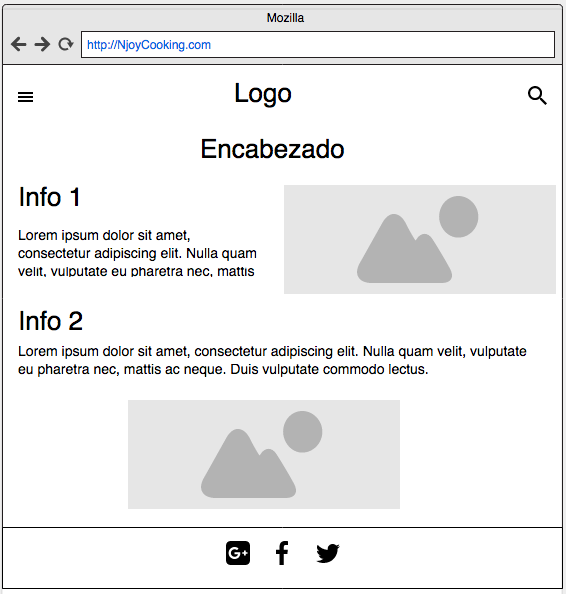
\includegraphics[width=1.0\textwidth]{imagenes/detalle-blog.png}
\caption{Detalle de noticia}
\label{detalle-blog}
\end{center}
\end{figure}

\begin{figure}
\begin{center}
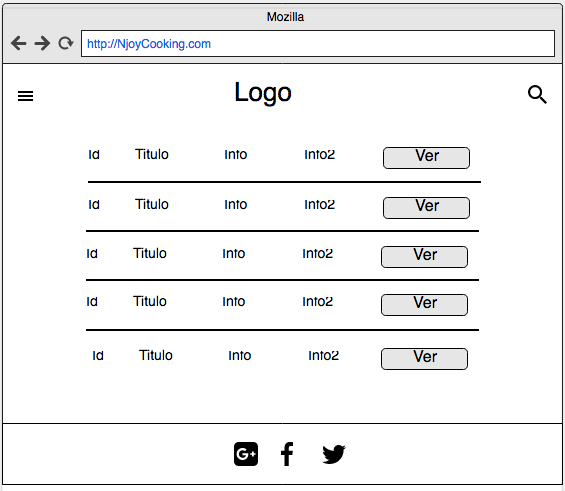
\includegraphics[width=1.0\textwidth]{imagenes/listado-admin.png}
\caption{Listado de elementos}
\label{listado-admin}
\end{center}
\end{figure}

Inicialmente se llevan a cabo unos bocetos de la web mediante mockups para saber como se va a organizar el contenido de la aplicación.

\vspace{5 mm}

Cualquier empresa que se encuentre en el mundo de las aplicaciones web sabe que una landing, es la mejor forma de promocionar el producto o marca que se quiere dara conocer. Por eso a la página inicial donde el usuario accederá será una landing donde se mostrará información acerca de los servicios que ofrece la web.

\vspace{5 mm}

Como se observa en el boceto(figura \ref{landing}) la landing tiene un diseño sencillo y usable. En esta página se mostrarán una series de secciones informativas acerca de los contenidos disponibles de la web y otras informaciones relevantes. Las secciones irán acompañadas de una imagen de fondo, un texto informativo y un botón que te dirige a la página correspondiente.

\vspace{5 mm}

La cabecera de la landing, que será común a todas las páginas de la web, tendrá un diseño responsive para todas las resoluciones. El menú será desplegable de forma que al pulsar sobre el icono de  la hamburguesa se verán todas las secciones por las que se podrá navegar por la web. Este menú mobile se ha aplicado para la resolución de escritorio ya que favorecía a conseguir una mayor limpieza de la interfaz,no empeoraba su usabilidad y le daba un aspecto más minimalista. Además de este menú en la cabecera encontraremos el logo de la web y un buscador global de la web. Esta cabecerá siempre estará fija para favorecer la usabilidad al usuario.

\vspace{5 mm}

Por último, el footer o pie de página, otro elemento común a todas las páginas. En esta sección se mostrarán las distintas redes sociales de la empresa, los textos legales(copyright,privacidad) y el logo de la web.


\vspace{5 mm}

La siguiente página, es la del mapa (figura \ref{mapa}). En esta página se mostraban un mapa con los marcadores de las recetas geoposiconadas. El diseño de esta página es muy sencillo ya que además de los elementos comunes de cabecera y pie, en el contenido se muestra un elemento con el mapa que va a mostrar la información.

\vspace{5 mm}

La próxima sección, es la sección del blog que se compone de dos páginas: el listado de noticias y el detalle de noticia. En el listado de noticias(figura \ref{listado-blog}), el primer elemento que se mostrará será un encabezado con una foto y descripción de la sección del blog. A continuación se mostrarán un listado con las diferentes noticias del blog y en cada una se mostrará un foto, un título y un resumen. Para esta sección la disposición de los elementos de la notícia en movil cambiará colocando los elementos en una sola columna en vez de dos como se muestran en tablet y pc.

\vspace{5 mm}

En el detalle de la receta(figura \ref{detalle-blog}) se muestra toda la información asociada a esa noticia. El primer elemento que aparece es el encabezado de la noticia donde se muestra su título y una foto de fondo. A continuación se muestra en dos columnas la información de la receta, una columna con un primer bloque de información y la segunda con la imagen principal de la noticia. Después se muestran los demás bloques de información en una sola columna y por último se muestran otra fotos asociadas a la noticia. Al final de la noticia se muestra un formulario para escribir comentarios asociados a la noticia y un listado con los comentarios que tiene la noticia. La estructura del contenido cambia para la resolución móvil mostrando todo el contenido en una columna.

\vspace{5 mm}

Si el usuario que accede a la página esta registrado, aparecerán nuevas secciones disponibles. Estas secciones serán vistas como listados de elementos(figura \ref{listado-admin}), se usaran para mostrar cualquier tipo de datos que visualice el usuario registrado. La información se listará en una disposición de tabla, con el contenido del elemento(id,titulo,etc) y un botón para ver el detalle. La presentación de este contenido es mucho más simple, que el listado para los usuarios no registrados, ya que esta sección tiene que ser mucho más pragmática y menos visual.

\vspace{5 mm}

\textbf{Paleta de Colores}

\vspace{5 mm}

\begin{figure}
\begin{center}
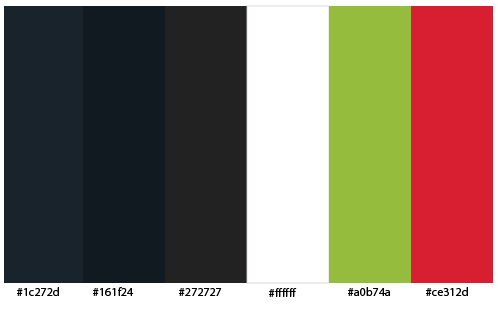
\includegraphics[width=1.0\textwidth]{imagenes/paleta.png}
\caption{Paleta de Colores}
\label{paleta}
\end{center}
\end{figure}

Para la aplicación se ha seleccionado una paleta de colores(\ref{paleta}) con el programa spectrum. Se ha elegido una gama de azules y grises oscuros que dan un aspecto de seriedad y confianza. También se utilizan una series de colores mas vivos como el verde y el rojo que se utilizan para los botones, pequeños detalles y resaltar los textos para dar una aspecto más vivo.


\subsection{Implementación de la arquitectura}

\begin{figure}
\begin{center}
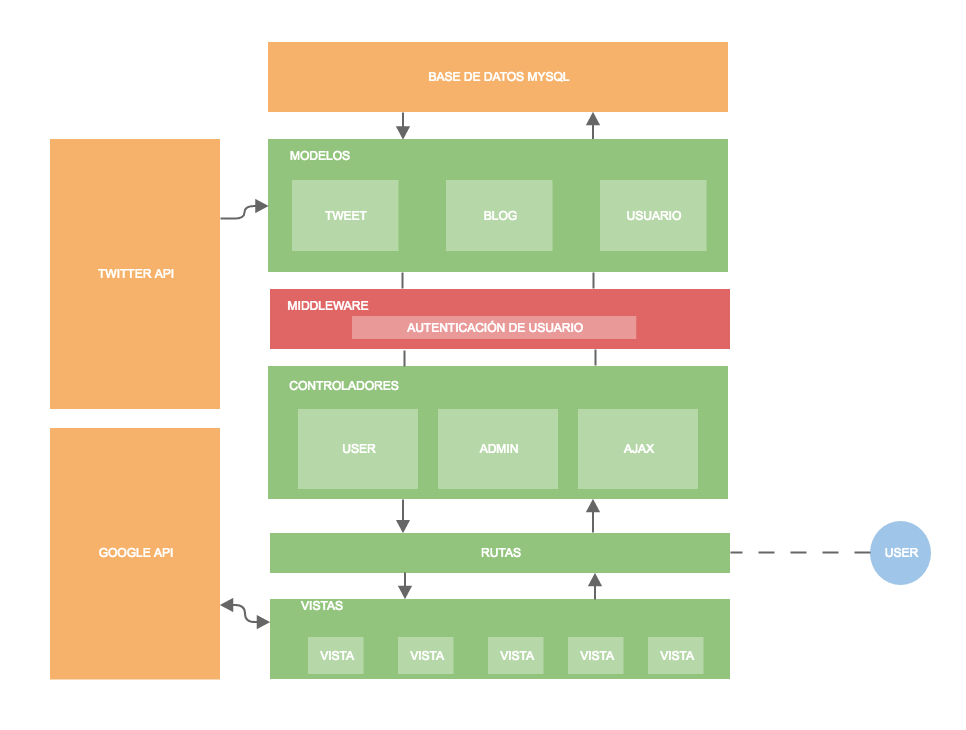
\includegraphics[width=1.0\textwidth]{imagenes/implementacion-arquitectura.png}
\caption{Arquitectura específica}
\label{implement-arch}
\end{center}
\end{figure}

En el segundo sprint del proyecto, se lleva acabo un esquema específico de la arquitectura usada para la aplicación. En este esquema de arquitectura ya no es tan general, se especifican detalladamente cada una de las capas de la arquitectura,se enumeran cada uno de los elementos que se va a componer y se detallan cada una de las APIs externas empleadas.

\vspace{5 mm}

En la figura \ref{implement-arch} se observa un esquema detallado de como se ha implementado la arquitectura de la aplicación. A continuación se procede a profundizar en cada una de las capas de la arquitectura.

\vspace{5 mm}

El usuario que navegue por la aplicación, accederá a las diferentes páginas de la web por medio de una ruta que introduzca en el navegador. Una vez introducida la ruta comienza el flujo de información de la aplicación.

\vspace{5 mm}

Con la ruta introducida, la aplicación nos manda al controlador correspondiente para obtener la información. Para organizar mejor la información, se crean tres controladores:

\begin{itemize}

\item \textbf{SiteController}: El controlador para manejar la información del usuario no registrado. Este controlador tendrá métodos para renderizar las partes de la web que son visibles para todo tipo de usuario, desde la landing page hasta el mapa, pasando por el blog

\item \textbf{AdminController}: Controlador que maneja el contenido que visualiza el administrador. Las páginas de listado de contenido y detalle que se usa el administrador para manipular la información se manejaran mediante este controlador 

\item \textbf{AjaxController}: en este controlador se manejarán todos los datos realizados con peticiones ajax. Apartados como los comentarios, utilizarán peticiones ajax para guardar la información en la base de datos y no tener que recargar la página.

\end{itemize}


En los controladores se hace uso de los diferentes modelos de datos de la aplicación. Los modelos generalmente se corresponden con una tabla de la base de datos. Para cada objeto de datos se crea la clase php(el Modelo) donde se encuentran los métodos que insertan, borran o actualizan la información de su tabla correspondiente. Por ejemplo, el modelo Tweets es la clase donde están definidos los métodos que guardan toda la información de los tweets recogidos.

\vspace{5 mm}


Para comprobar la autenticación del cliente, y que cualquier usuario no pueda acceder a partes de la web que solo están disponibles para el administrador, se implementa una capa intermedia entre los controladores y los modelos llamada middleware.








